\documentclass[UTF8,12pt]{article}

\usepackage[utf8]{inputenc}
\usepackage{ctex}
\usepackage{amsmath,amsfonts,amssymb}
\usepackage{graphicx,epsfig,subfig}
\usepackage{makeidx,hyperref}
\usepackage{geometry}
\usepackage{listings}
\usepackage[linesnumbered,boxed]{algorithm2e}
\usepackage{xcolor}

\geometry{scale=0.8}

%\setlength{\lineskip}{\baselineskip}
\setlength{\parskip}{0.5\baselineskip}

\title{谱元法笔记}
\author{flag}
\date{\today}

\begin{document}
    
\maketitle

目前的代码可以求解这两个问题:

特征值问题
\begin{eqnarray}
- \Delta u(\mathbf{x}) + V(\mathbf{x}) u(\mathbf{x}) = \lambda u(\mathbf{x}) \qquad \mathbf{x} \in \Omega \\
\frac{\partial u}{\partial n}(\mathbf{x}) + h u(\mathbf{x}) = 0 \qquad \mathbf{x} \in \partial \Omega
\end{eqnarray}

源项问题
\begin{eqnarray}
- \Delta u(\mathbf{x}) + V(\mathbf{x}) u(\mathbf{x}) = 1 \qquad \mathbf{x} \in \Omega \\
\frac{\partial u}{\partial n}(\mathbf{x}) = g \qquad \mathbf{x} \in \partial \Omega
\end{eqnarray}

一维的情况时,区域$\Omega=[0,1]$被均匀分成$M$个区间,二维时,$V(x)$区域$\Omega=[0,1] \times [0,1]$被均匀分成$M_1 \times M_2$个方格。在每个方格上$V(\mathbf{x})$是分片常数,而且大于0。

\section{comment1}
    
在相同的位势V的选取下,比较Robin边界条件的解与Dirichlet边界条件的解,找到一个例子说明两者的landscape和eigenmodes都相差很大。这样可以说明我们研究的重要性。

Dirichlet边界条件的程序正在写,过几天就可以完成。

\section{comment2}

让V在每个方格内取[0,1]上均匀分布的随机数。比较该结果与V在每个方格内取{0,1}值Bernoulli分布的异同。

取K为8000,V取均匀分布的随机数,Neumman边界条件(h和g都是0)。得到图\ref{fig1}

\begin{figure}[htbp]
\centering
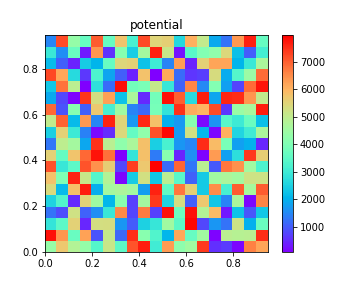
\includegraphics[width=0.3\linewidth]{../pics/v1}
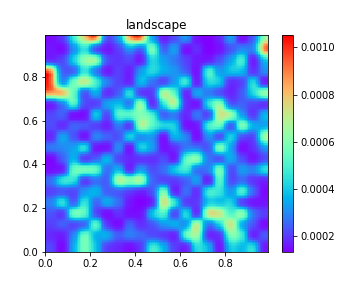
\includegraphics[width=0.3\linewidth]{../pics/w1}
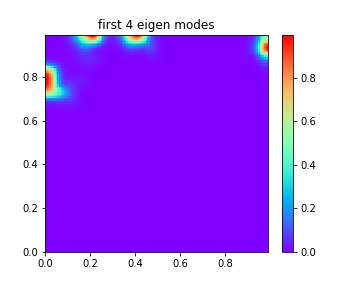
\includegraphics[width=0.3\linewidth]{../pics/u1}
\caption{K=8000, Uniform distribution}
\label{fig1}
\end{figure}

取K为8000,V取Bernoulli分布的随机数,V取0的概率p=0.5(保证均值相同),Neumman边界条件(h和g都是0)。得到图\ref{fig2}

\begin{figure}[htbp]
    \centering
    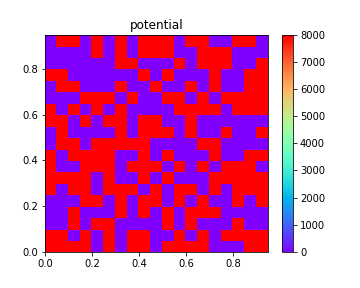
\includegraphics[width=0.3\linewidth]{../pics/v2}
    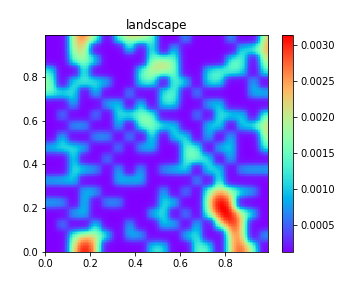
\includegraphics[width=0.3\linewidth]{../pics/w2}
    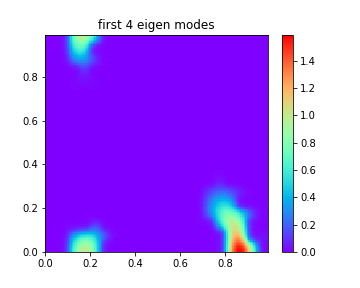
\includegraphics[width=0.3\linewidth]{../pics/u2}
    \caption{K=8000, p=0.5, Bernoulli distribution}
    \label{fig2}
\end{figure}

可以看出,均匀分布让特征函数的峰局部化更加明显。


\section{comment3}

你上次提到的想法应该继续挖掘:找到一个阈值,将landscape大于这个阈值的子区域找出来,研究该子区域的分块情况。例如,这个阈值可以取作1/[3(lambda+alpha+beta)]。

把$\{x: (\lambda+\alpha+\beta)w(x) < 1\}$的区域涂黑,其它区域涂白。并把它和eigenmode对比,得到图\ref{fig11}。

\begin{figure}[htbp]
    \centering
    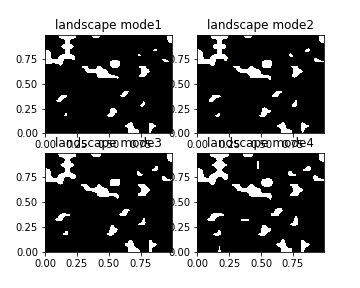
\includegraphics[width=0.45\linewidth]{../pics/wm11}
    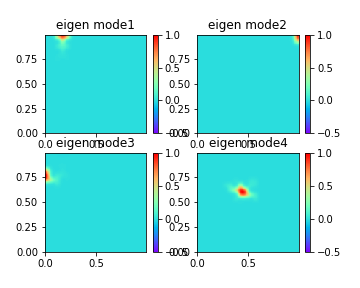
\includegraphics[width=0.45\linewidth]{../pics/u11}
    \caption{K=8000, p=0.3, Bernoulli distribution}
    \label{fig11}
\end{figure}

从图中来看,eigenmode的峰值位置确实被限制在了涂白的地方。但是黑白这样的图有点难看,不如valley line的图漂亮。但是从另一种角度看,valley line只是告诉我们特征函数峰的划分,而黑白的图不仅可以看出特征函数在哪有峰,还可以看出特征函数在哪一定没有峰。

\section{comment4}

在V取{0,1}值Bernoulli分布时,二维情形取0的概率p有临界值0.59。p大于这个临界值时,子区域应该是连成一片的;小于这个临界值时,子区域应该分成很多小块。尝试验证这个结果。

在临界值附近选取p的值,得到图\ref{fig3}和图\ref{fig4}。

\begin{figure}[htbp]
    \centering
    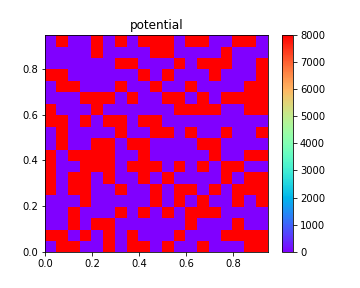
\includegraphics[width=0.3\linewidth]{../pics/v3}
    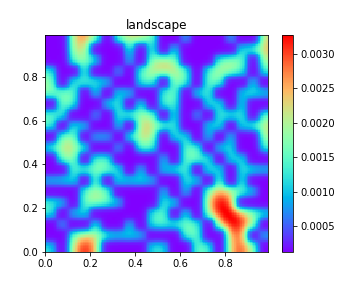
\includegraphics[width=0.3\linewidth]{../pics/w3}
    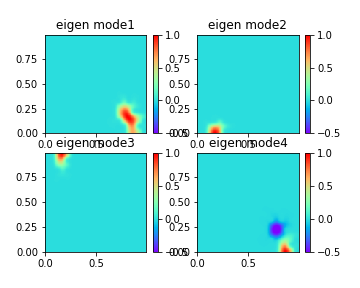
\includegraphics[width=0.3\linewidth]{../pics/u3}
    \caption{K=8000, p=0.58, Bernoulli distribution}
    \label{fig3}
\end{figure}

\begin{figure}[htbp]
    \centering
    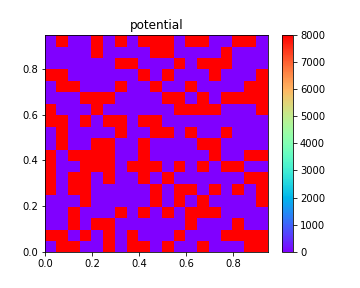
\includegraphics[width=0.3\linewidth]{../pics/v4}
    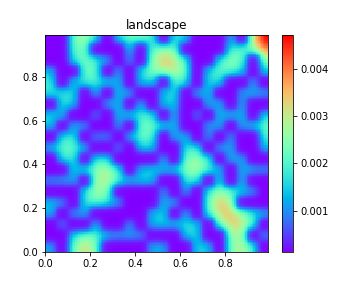
\includegraphics[width=0.3\linewidth]{../pics/w4}
    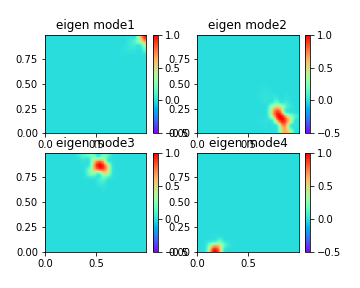
\includegraphics[width=0.3\linewidth]{../pics/u4}
    \caption{K=8000, p=0.60, Bernoulli distribution}
    \label{fig4}
\end{figure}

两张图用的随机数种子是相同的,所以大致看上去没什么区别。仔细观察可以发现,他们的连通程度确实不一样。

\section{comment5}

尝试画出landscape的valley line。并研究valley line分出的块和Comment 3中分出的块的关系。

valley line的程序正在写,过几天就可以完成。

\section{comment6}

调整p与K的取值,使得Comment 3与Comment 5可以实现更好的分块。

改变不同的p,画出comment 3中的图,得到图\ref{fig12},图\ref{fig13}和图\ref{fig14}。

\begin{figure}[htbp]
    \centering
    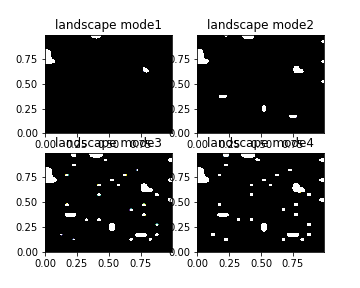
\includegraphics[width=0.45\linewidth]{../pics/wm12}
    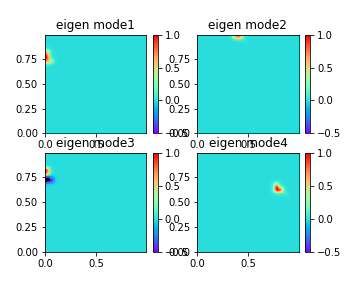
\includegraphics[width=0.45\linewidth]{../pics/u12}
    \caption{K=8000, p=0.1, Bernoulli distribution}
    \label{fig12}
\end{figure}

\begin{figure}[htbp]
    \centering
    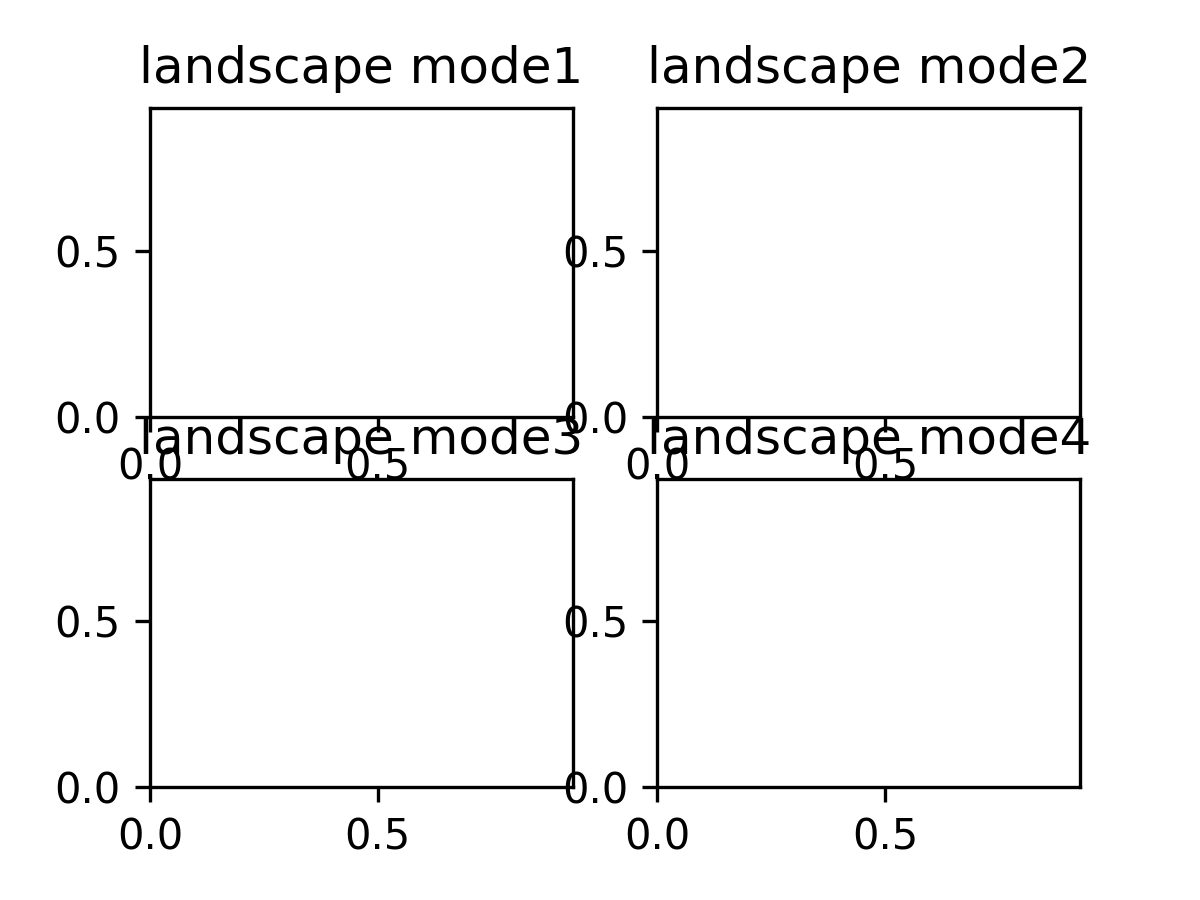
\includegraphics[width=0.45\linewidth]{../pics/wm13}
    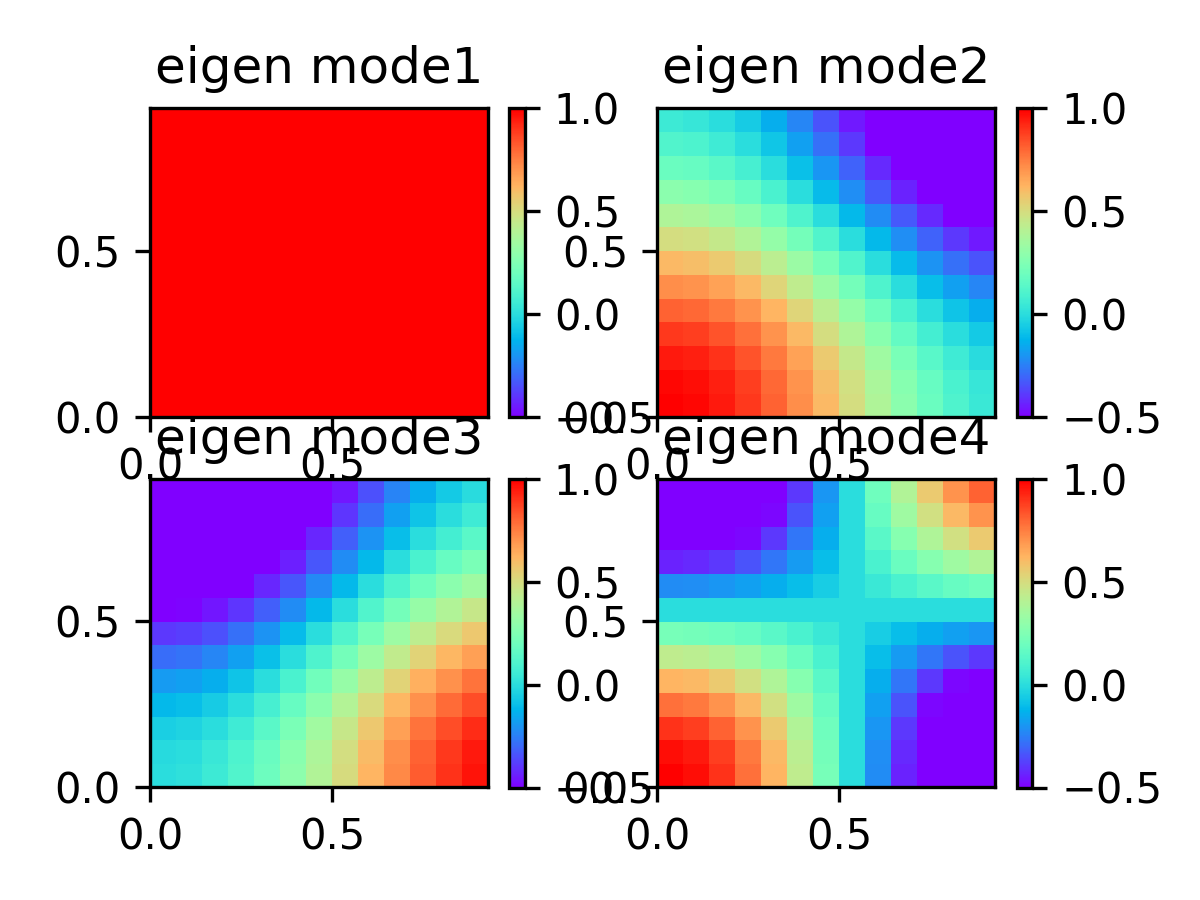
\includegraphics[width=0.45\linewidth]{../pics/u13}
    \caption{K=8000, p=0.2, Bernoulli distribution}
    \label{fig13}
\end{figure}

\begin{figure}[htbp]
    \centering
    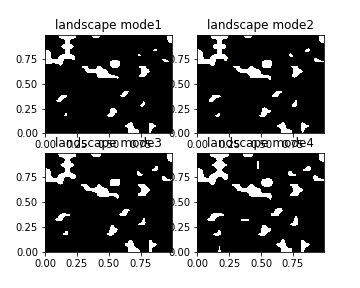
\includegraphics[width=0.45\linewidth]{../pics/wm11}
    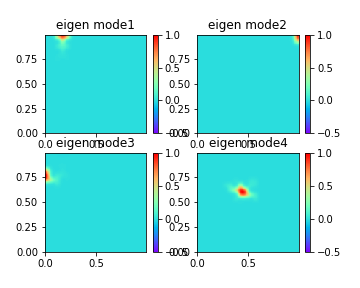
\includegraphics[width=0.45\linewidth]{../pics/u11}
    \caption{K=8000, p=0.3, Bernoulli distribution}
    \label{fig14}
\end{figure}

根据试验的结果,p越小,K越大,局部化越明显。分块也更准确。

\section{comment7}

在V取{0,1}值的Bernoulli分布时,让K趋于无穷,比较K很大时候landscape的分块与{x: V(x)=0}的连通分支的关系。

不断增大K,在同一组随机数下求解问题。得到图\ref{fig5},图\ref{fig6}和图\ref{fig7}。

\begin{figure}[htbp]
    \centering
    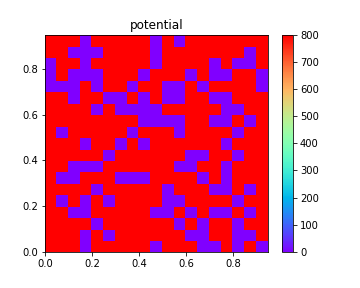
\includegraphics[width=0.3\linewidth]{../pics/v5}
    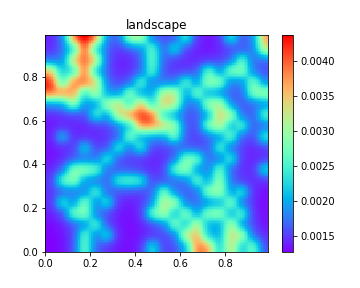
\includegraphics[width=0.3\linewidth]{../pics/w5}
    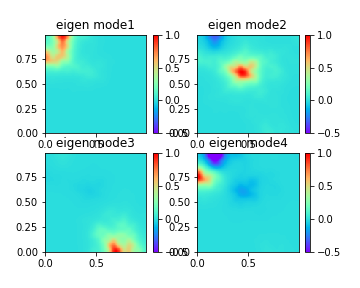
\includegraphics[width=0.3\linewidth]{../pics/u5}
    \caption{K=800, p=0.30, Bernoulli distribution}
    \label{fig5}
\end{figure}

\begin{figure}[htbp]
    \centering
    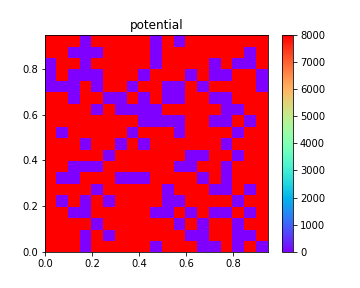
\includegraphics[width=0.3\linewidth]{../pics/v6}
    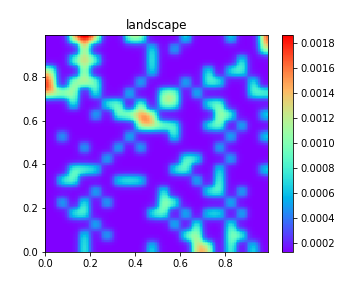
\includegraphics[width=0.3\linewidth]{../pics/w6}
    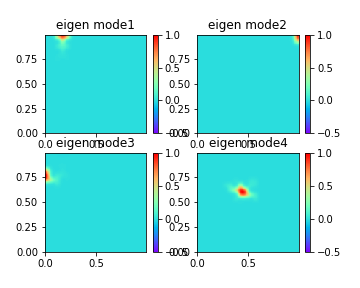
\includegraphics[width=0.3\linewidth]{../pics/u6}
    \caption{K=8000, p=0.30, Bernoulli distribution}
    \label{fig6}
\end{figure}

\begin{figure}[htbp]
    \centering
    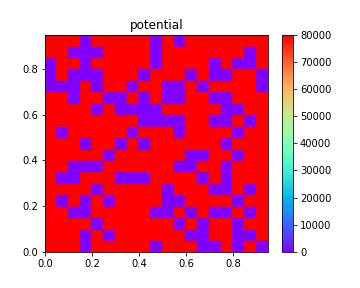
\includegraphics[width=0.3\linewidth]{../pics/v7}
    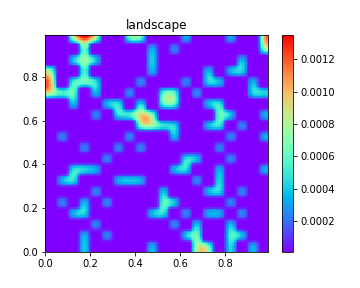
\includegraphics[width=0.3\linewidth]{../pics/w7}
    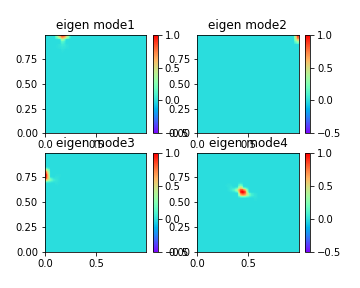
\includegraphics[width=0.3\linewidth]{../pics/u7}
    \caption{K=80000, p=0.30, Bernoulli distribution}
    \label{fig7}
\end{figure}

可以看出,K越大时,landscape的局部化现象会更加明显,特征函数的局部化也会更加明显。在K很大的时候,landscape会呈现出和K类似的形状,在V(x)间断的地方,landscape就会变得陡峭。

\section{comment8}

在V取[0,1]上均匀分布的随机数时,验证当K趋于无穷时,eigenmode集中在V的最小值附近。

不断增大K,在同一组随机数下求解问题。得到图\ref{fig8},图\ref{fig9}和图\ref{fig10}。

\begin{figure}[htbp]
    \centering
    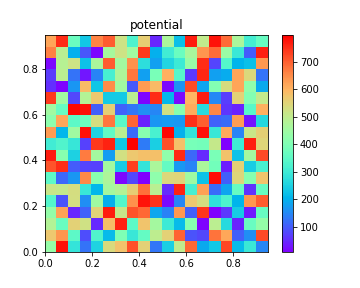
\includegraphics[width=0.3\linewidth]{../pics/v8}
    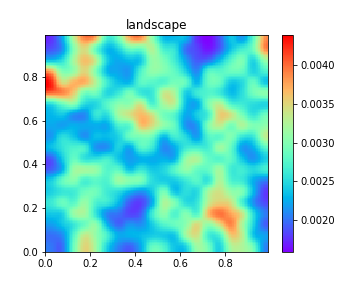
\includegraphics[width=0.3\linewidth]{../pics/w8}
    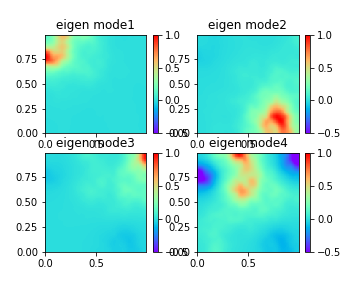
\includegraphics[width=0.3\linewidth]{../pics/u8}
    \caption{K=800, Uniform distribution}
    \label{fig8}
\end{figure}

\begin{figure}[htbp]
    \centering
    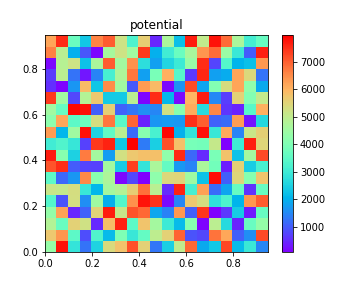
\includegraphics[width=0.3\linewidth]{../pics/v9}
    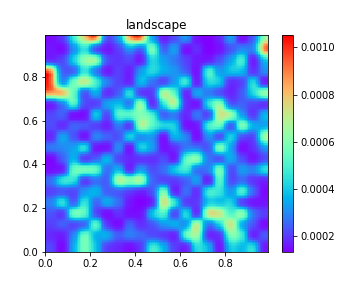
\includegraphics[width=0.3\linewidth]{../pics/w9}
    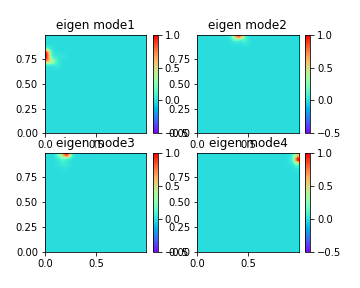
\includegraphics[width=0.3\linewidth]{../pics/u9}
    \caption{K=8000, Uniform distribution}
    \label{fig9}
\end{figure}

\begin{figure}[htbp]
    \centering
    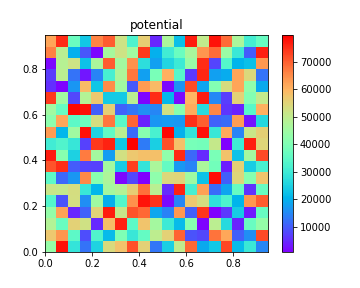
\includegraphics[width=0.3\linewidth]{../pics/v10}
    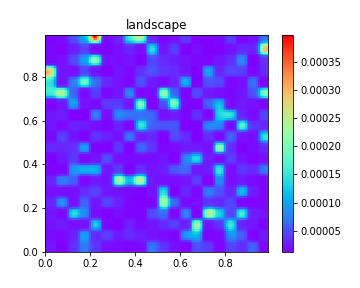
\includegraphics[width=0.3\linewidth]{../pics/w10}
    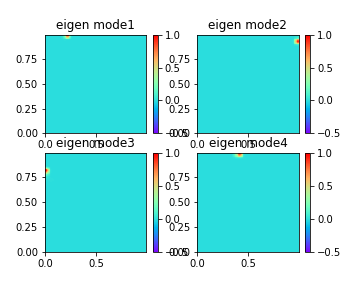
\includegraphics[width=0.3\linewidth]{../pics/u10}
    \caption{K=80000, Uniform distribution}
    \label{fig10}
\end{figure}

均匀分布下,特征函数随K增大而局部化的现象比0-1分布时更加明显。但是eigenmode集中在V的最小值附近的现象还不是很明显。
    
\end{document}